\documentclass[aps,pra,twocolumn,reprint,floatfix,amsmath,amssymb]{revtex4-2}

\usepackage{graphicx}
\usepackage{booktabs}
\usepackage{siunitx}
\usepackage[colorlinks=true,linkcolor=blue,citecolor=blue,urlcolor=blue]{hyperref}

\begin{document}

\title{Expanded Study of Parameterized Multitone Waveform Families for Residual-Z Cancellation}
\author{GitHub Copilot}
\affiliation{cQED Autonomous Research Platform}
\date{\today}

\begin{abstract}
We study whether richer multitone waveform families can suppress the coherent blockwise residual-$Z$ error that limits arbitrary Fock-conditional qubit rotations in a dispersive qubit--cavity model. The comparison keeps the same qubit-first \texttt{cqed\_sim} logical-subspace workflow used in the completed baseline study and changes only the waveform family. Five families are compared: the built-in Gaussian targeted-subspace multitone baseline, a symmetric two-segment family, an explicit echoed family with a mid-sequence qubit $X_\pi$ pulse, a complex-envelope family, and a basis-expanded family. The expanded sweep covers $48$ cases and $240$ waveform-family rows spanning $N_{\mathrm{active}} = 2,3,4$, $|\chi|T/2\pi \in \{3,5\}$, both the $\chi$-only and $\chi+\chi'$ models, one smooth structured target family, and three random block targets per configuration.

The results separate sharply by target class. On smooth structured targets, the best single-segment richer families improve fidelity only marginally over the baseline: the best overall case reaches average gate fidelity $0.874158$ versus $0.873359$ for the baseline, while the echoed family fails badly. On random targets, however, the echoed family wins $23$ of $36$ cases, increasing mean fidelity from $0.247163$ to $0.321155$ and simultaneously reducing mean residual-$Z$ error from $0.980429$ rad to $0.627334$ rad and mean transverse coherent error from $1.790404$ rad to $1.590729$ rad. The main conclusion is therefore not that residual-$Z$ cancellation alone solves the control problem, but that the hard random-target regime benefits from genuinely multi-segment structure, whereas smooth structured targets remain best served by modest single-segment envelope refinements.
\end{abstract}

\maketitle

\section{Introduction}
The earlier arbitrary conditional-rotation baseline study in this repository established a strong negative result for the standard Gaussian simultaneous multitone SQR ansatz: over a finite active Fock window, arbitrary block-diagonal conditional qubit rotations do not reach high fidelity even when off-target population transfer is already small. That finding narrowed the next question. Is the dominant obstruction mainly a residual blockwise $Z$ mismatch that can be cancelled by a richer waveform family, or does the failure reflect a broader coherent-control limitation?

This follow-up study keeps the same dispersive transmon--cavity model, the same qubit-first logical basis ordering, and the same targeted-subspace diagnostics, but expands the waveform family set. The design goal is pragmatic rather than formal optimal control: identify whether modestly richer, still-structured waveform families materially improve the hard arbitrary-target cases without abandoning the multitone framework already available in \texttt{cqed\_sim}~\cite{cqed_sim}.

\section{System and Methods}
\subsection{Hamiltonian}
The simulations use the closed-system dispersive qubit--cavity model implemented in \texttt{cqed\_sim}. In the frame conventions used here, the effective Hamiltonian is summarized by
\begin{equation}
\frac{H}{\hbar} = \omega_c a^\dagger a + \frac{\omega_q}{2}\sigma_z + \chi a^\dagger a \, |e\rangle\langle e| + \chi' a^\dagger a (a^\dagger a - 1) \, |e\rangle\langle e|,
\end{equation}
with qubit-first tensor ordering. The logical basis is therefore
\begin{equation}
(|g,0\rangle, |e,0\rangle, |g,1\rangle, |e,1\rangle, \ldots).
\end{equation}
The main comparison sets the cavity self-Kerr to zero and uses a two-level qubit model so the targeted-subspace diagnostics remain identical across all waveform families.

\subsection{Simulation Parameters}
Table~\ref{tab:params} lists the fixed numerical parameters used throughout the expanded sweep.

\begin{table}[t]
    \centering
    \caption{Fixed model and numerical parameters for the expanded waveform-family comparison.}
    \label{tab:params}
    \begin{tabular}{@{}lll@{}}
        \toprule
        Parameter & Value & Unit \\
        \midrule
        $\omega_q/2\pi$ & 6.150 & GHz \\
        $\omega_c/2\pi$ & 5.241 & GHz \\
        $\alpha/2\pi$ & -255 & MHz \\
        $\chi/2\pi$ & -2.84 & MHz \\
        $\chi'/2\pi$ & -21 & kHz \\
        $K/2\pi$ & 0 & kHz \\
        $\Delta t$ & 4 & ns \\
        $N_{\mathrm{active}}$ & 2, 3, 4 & manifolds \\
        $N_{\mathrm{cav}}$ & $N_{\mathrm{active}} + 2$ & levels \\
        $N_{\mathrm{tr}}$ & 2 & levels \\
        $|\chi|T/2\pi$ & 3, 5 & dimensionless \\
        \bottomrule
    \end{tabular}
\end{table}

\subsection{Computational Approach}
The baseline family is optimized with \texttt{optimize\_targeted\_subspace\_multitone}. Four local extensions are then compared using the same simulator and logical-subspace analysis stack:
\begin{enumerate}
    \item baseline Gaussian multitone,
    \item symmetric two-segment multitone,
    \item echoed multitone with an explicit mid-sequence Gaussian $X_\pi$ pulse,
    \item complex-envelope multitone,
    \item basis-expanded multitone.
\end{enumerate}
The structured target set uses the smooth family $C$ already defined in the study utilities. The hard targets use Haar-random blockwise SU(2) rotations (family $D$), with three seeds per $(\text{model}, N_{\mathrm{active}}, T)$ point. The richer families are optimized locally with Powell search over sampled-envelope parameters while keeping the same tone set extracted from the optimized baseline. For every case, we record average gate fidelity, restricted process fidelity, residual-$Z$ error from the blockwise error-unitary rotation vector, transverse coherent error, state-level validation on cavity-superposition probes, and saved waveform samples in both JSON and NPZ formats.

\section{Results}
\subsection{Global Family Averages}
Figure~\ref{fig:familymeans} summarizes the averages over all $240$ rows. The three single-segment families remain tightly clustered: basis-expanded, complex-envelope, and the baseline differ in mean fidelity by only $1.5 \times 10^{-3}$. The symmetric two-segment family lowers mean residual-$Z$ modestly, but it does not translate that reduction into better overall fidelity. The echoed family is the clear outlier: it achieves the lowest mean residual-$Z$ error across the full grid, but also the worst mean fidelity and the largest mean transverse error when structured and random targets are pooled together. That apparent contradiction is resolved only after separating the two target classes.

\begin{figure}[t]
    \centering
    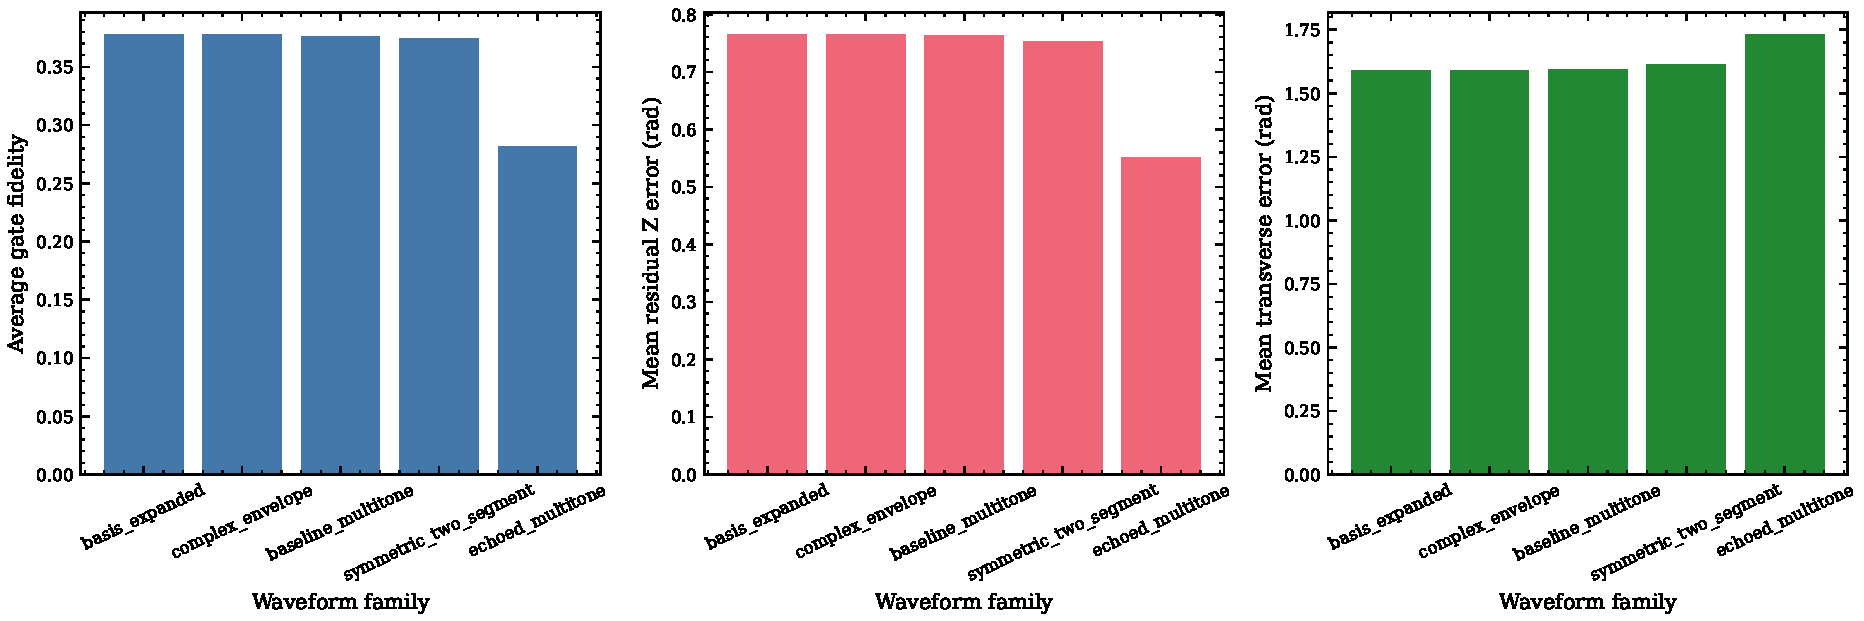
\includegraphics[width=\columnwidth]{../figures/family_metric_means.pdf}
    \caption{Expanded-study family means over all $240$ waveform-family rows. The single-segment families remain tightly grouped, while the echoed family strongly lowers mean residual-$Z$ error at the cost of much worse global average fidelity because it performs poorly on the structured targets.}
    \label{fig:familymeans}
\end{figure}

\subsection{Structured Targets: Only Marginal Single-Segment Gains}
For the smooth structured target family $C$, the single-segment richer families are only incremental improvements. Averaged over the structured subset, basis-expanded reaches mean fidelity $0.765097$, complex-envelope reaches $0.764993$, and the baseline reaches $0.763677$. The best overall structured point is the basis-expanded family in the $\chi + \chi'$ model at $N_{\mathrm{active}} = 2$ and $|\chi|T/2\pi = 5$, with average gate fidelity $0.874158$. This is only $7.99 \times 10^{-4}$ above the corresponding baseline value $0.873359$.

The structured-target scaling remains poor as the active window grows. The best fidelity falls from about $0.874$ at $N_{\mathrm{active}} = 2$ to about $0.781$ at $N_{\mathrm{active}} = 3$ and about $0.674$ at $N_{\mathrm{active}} = 4$ in the $\chi$-only model. The same qualitative decline appears in the $\chi + \chi'$ model. In this regime, the control problem still looks like a limited-improvement refinement of the baseline ansatz rather than a qualitative recovery.

The echoed family is actively harmful on the structured set. Its structured-target mean fidelity is only $0.164414$, compared with $0.763677$ for the baseline. In the same subset, the mean residual-$Z$ error increases from $0.114305$ rad to $0.323200$ rad and the mean transverse error increases from $1.007713$ rad to $2.153126$ rad. The present global echo pulse is therefore not a generic structured-target improvement.

\subsection{Random Targets: Echo Helps the Hard Cases}
The random block targets tell a different story. Here the echoed family wins $23$ of the $36$ random-target cases when cases are judged by average gate fidelity. Relative to the baseline, the echoed family improves the random-target mean fidelity from $0.247163$ to $0.321155$, lowers the mean residual-$Z$ error from $0.980429$ rad to $0.627334$ rad, and lowers the mean transverse error from $1.790404$ rad to $1.590729$ rad.

This is not a purely residual-$Z$ story. Figure~\ref{fig:tradeoffs} shows that the random-target echoed gains correlate with simultaneous reductions in both coherent-error components, whereas the complex-envelope and basis-expanded families remain close to the baseline in both coordinates. The hardest random-target improvements are substantial in the $\chi$-only model: at $N_{\mathrm{active}} = 4$, the median random-target fidelity rises from $0.207933$ for the baseline to $0.400839$ for the echoed family. In the $\chi + \chi'$ model, the improvement is more modest but still present at $N_{\mathrm{active}} = 4$, where the median rises from $0.117406$ to $0.160696$.

\begin{figure}[t]
    \centering
    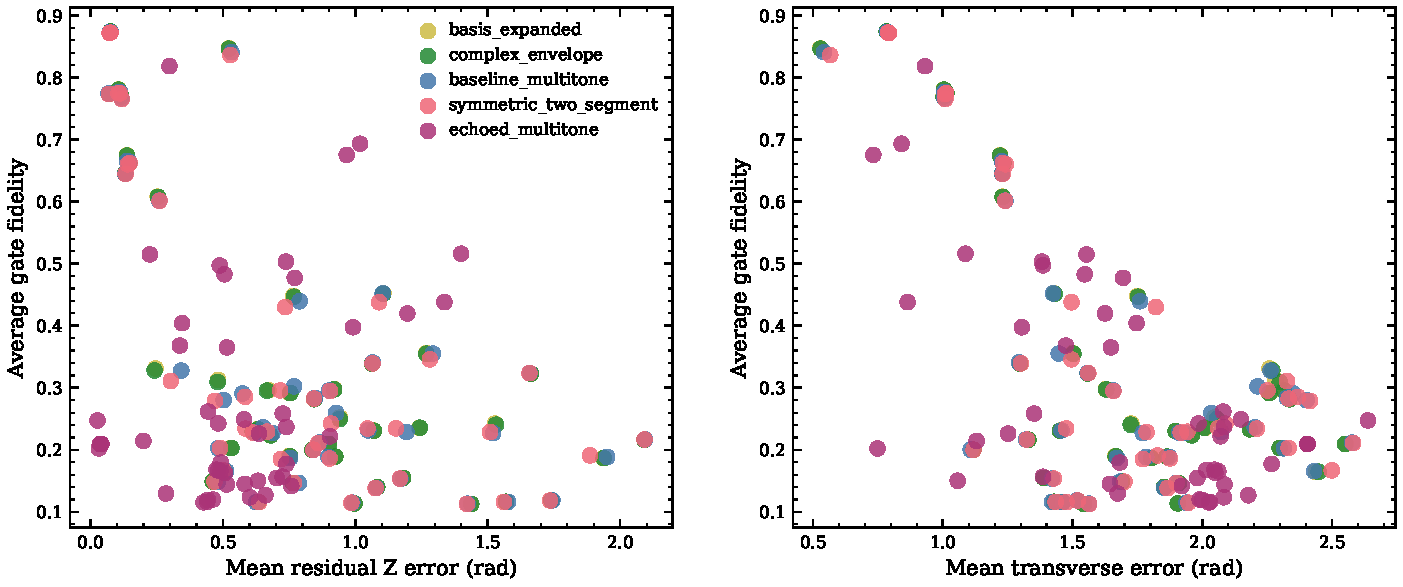
\includegraphics[width=\columnwidth]{../figures/fidelity_tradeoff_planes.pdf}
    \caption{Tradeoff planes for the expanded sweep. Left: average gate fidelity versus mean residual-$Z$ error. Right: average gate fidelity versus mean transverse error. The echoed family creates a separate cluster that improves many hard random targets while failing badly on the structured target set.}
    \label{fig:tradeoffs}
\end{figure}

\subsection{Case-Level Structure and Spectral Diversity}
The full case-by-family fidelity map is included in the appendix. The most important pattern is that the structured target rows form a nearly flat high-fidelity band for the baseline, complex-envelope, and basis-expanded families, whereas the echoed family collapses on the same rows but frequently dominates in the random-target rows.

Representative spectra reinforce that these families are not minor parameter variations of one another. Figure~\ref{fig:spectra} shows a representative hard random case from the $\chi + \chi'$ model at $N_{\mathrm{active}} = 4$ and $|\chi|T/2\pi = 5$. The baseline and basis-expanded families remain relatively smooth, while the complex-envelope and symmetric two-segment families develop stronger localized sidebands. The echoed family instead spreads most of its power into a low-frequency-dominated profile because the explicit mid-sequence qubit echo changes the time-domain construction rather than merely the envelope coefficients.

\begin{figure}[t]
    \centering
    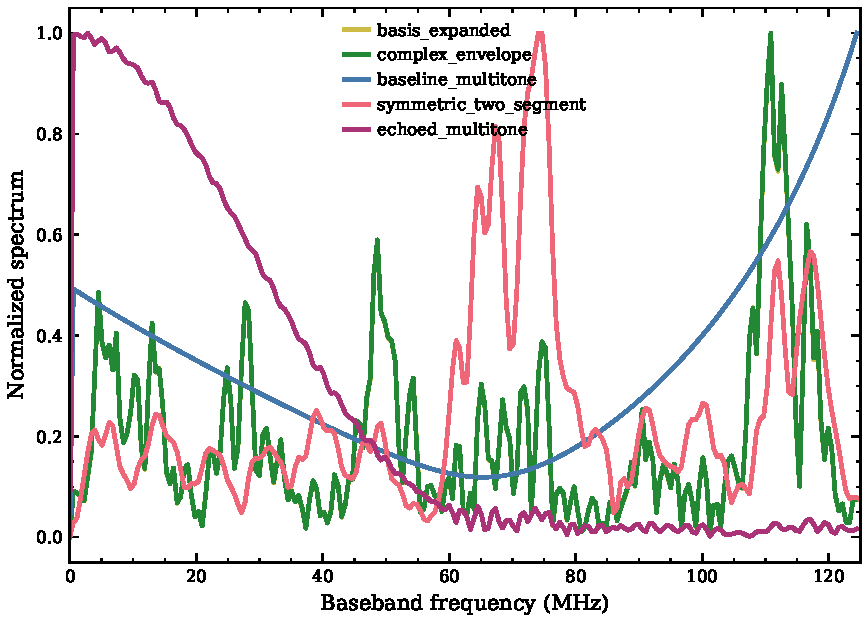
\includegraphics[width=\columnwidth]{../figures/representative_waveform_spectra.pdf}
    \caption{Representative normalized baseband spectra for a hard random case in the $\chi + \chi'$ model with $N_{\mathrm{active}} = 4$ and $|\chi|T/2\pi = 5$. The family-dependent spectral structure confirms that the richer families explore genuinely different control profiles rather than only small coefficient perturbations of the baseline waveform.}
    \label{fig:spectra}
\end{figure}

\section{Validation}
\subsection{Sanity Checks}
All simulations remained in the intended active subspace to numerical precision. Across the expanded sweep, leakage outside the target subspace stays at machine-zero levels, and the restricted unitarity error remains in the $10^{-6}$ range. The structured-target subset also provides an internal sanity check: the baseline, complex-envelope, and basis-expanded families agree closely on the easy cases, so the richer local optimizer is not inventing spurious large gains where none should exist.

\subsection{Convergence Analysis}
A full convergence campaign has not yet been completed. The present study fixes $\Delta t = \SI{4}{ns}$ and $N_{\mathrm{cav}} = N_{\mathrm{active}} + 2$ across all cases. The conclusions therefore rely on cross-family consistency at fixed numerics, not on a completed timestep or truncation sweep. This is sufficient for comparing the present waveform families to one another, but not yet for claiming full numerical convergence.

\subsection{Literature Comparison}
There is no direct external literature benchmark for this exact arbitrary block-target comparison. Instead, the relevant reference point is the completed repository baseline study, which has now been updated to record the same residual-$Z$/transverse decomposition. That internal apples-to-apples comparison supports the main conclusion here: the hard random-target gains from the echoed family are real within the present workflow, but they do not generalize to the smooth structured targets.

\section{Discussion}
The expanded sweep shows a two-regime control landscape. Smooth structured targets are already aligned well enough with the baseline multitone ansatz that only small gains are available from richer single-segment envelopes. In that regime, the main bottleneck appears to be the limited expressivity of simultaneous conditioned control as the active window grows, not a specific residual-$Z$ nuisance that can be echoed away.

The random-target regime is different. The echoed family improves fidelity precisely where the baseline and single-segment refinements fail most strongly, and it does so by reducing both residual-$Z$ and transverse coherent error. That matters because the earlier pilot already suggested that residual-$Z$ suppression alone was not enough. The expanded data sharpen that point: the hard-case improvement comes from changing the protocol structure, not from slightly better envelope shaping inside the same single-segment template.

At the same time, the current echo construction is clearly incomplete. A single global manifold-0 $X_\pi$ pulse is too blunt for the structured targets. The next useful question is therefore not whether echo helps in principle, but which manifold-aware or jointly optimized echoed protocol preserves the structured-case performance while keeping the random-case gains.

\section{Conclusion}
Five waveform families were compared over an expanded $48$-case sweep for arbitrary Fock-conditional qubit rotations. The best single-segment refinements, basis-expanded and complex-envelope, only slightly outperform the Gaussian baseline on smooth structured targets and do not change the qualitative scaling failure with larger active windows. The explicit echoed family, however, improves a majority of the hard random-target cases and reduces both residual-$Z$ and transverse coherent error there. The main conclusion is therefore split: structured targets remain a small-improvement single-segment problem, while hard random targets benefit from genuinely multi-segment protocol structure. Residual-$Z$ cancellation matters, but it is not the whole story.

\section{Limitations and Future Work}
\subsection{Known Limitations}
The richer families are implemented locally because \texttt{cqed\_sim} does not yet expose arbitrary sampled-envelope targeted-subspace optimization. The present echoed family uses a single global manifold-0 Gaussian $X_\pi$ pulse and is therefore only a first protocol sketch, not a polished echoed construction. The study remains closed-system, uses a two-level qubit model, and has not yet completed formal timestep or truncation convergence sweeps. The random ensemble is larger than the original pilot but still modest at three seeds per configuration.

\subsection{Suggested Improvements}
\begin{itemize}
    \item \textbf{[P1 | MEDIUM]} Add an upstream arbitrary-envelope targeted-subspace optimizer to \texttt{cqed\_sim} so richer families are optimized directly rather than through local wrappers.
    \item \textbf{[P2 | MEDIUM]} Replace the current global echo with a manifold-aware echoed protocol or a jointly optimized auxiliary-qubit sequence that can preserve structured-target performance.
    \item \textbf{[P2 | MEDIUM]} Promote the current scalarized local objective into a Pareto analysis over fidelity, residual-$Z$, and transverse coherent error.
    \item \textbf{[P2 | LOW]} Extend the scaling sweep to $N_{\mathrm{active}} = 5$ and increase the random-target ensemble to at least ten seeds per configuration.
    \item \textbf{[P2 | MEDIUM]} Add formal convergence and open-system validation so the present comparative findings can be upgraded to production-quality numerical claims.
\end{itemize}

\subsection{Open Questions}
Why does the present echo help the random-target regime while failing so badly on the smooth structured targets? Is the gain robust under a larger random ensemble, or is it tied to the current global-echo calibration? And, more generally, which coherent-error component should be treated as the real bottleneck once multi-segment structure is allowed?

\bibliographystyle{apsrev4-2}
\bibliography{references}

\appendix

\section{Detailed Results and Data}
The complete flat table is stored in \path{data/study_results.csv}, with matching JSON summaries in \path{data/study_results.json} and \path{data/study_summary.json}. Figure~\ref{fig:appendix_heatmap} shows the full case-by-family fidelity heatmap, and Fig.~\ref{fig:appendix_errorplane} shows the full residual-$Z$ versus transverse-error cloud.

\begin{figure*}[t]
    \centering
    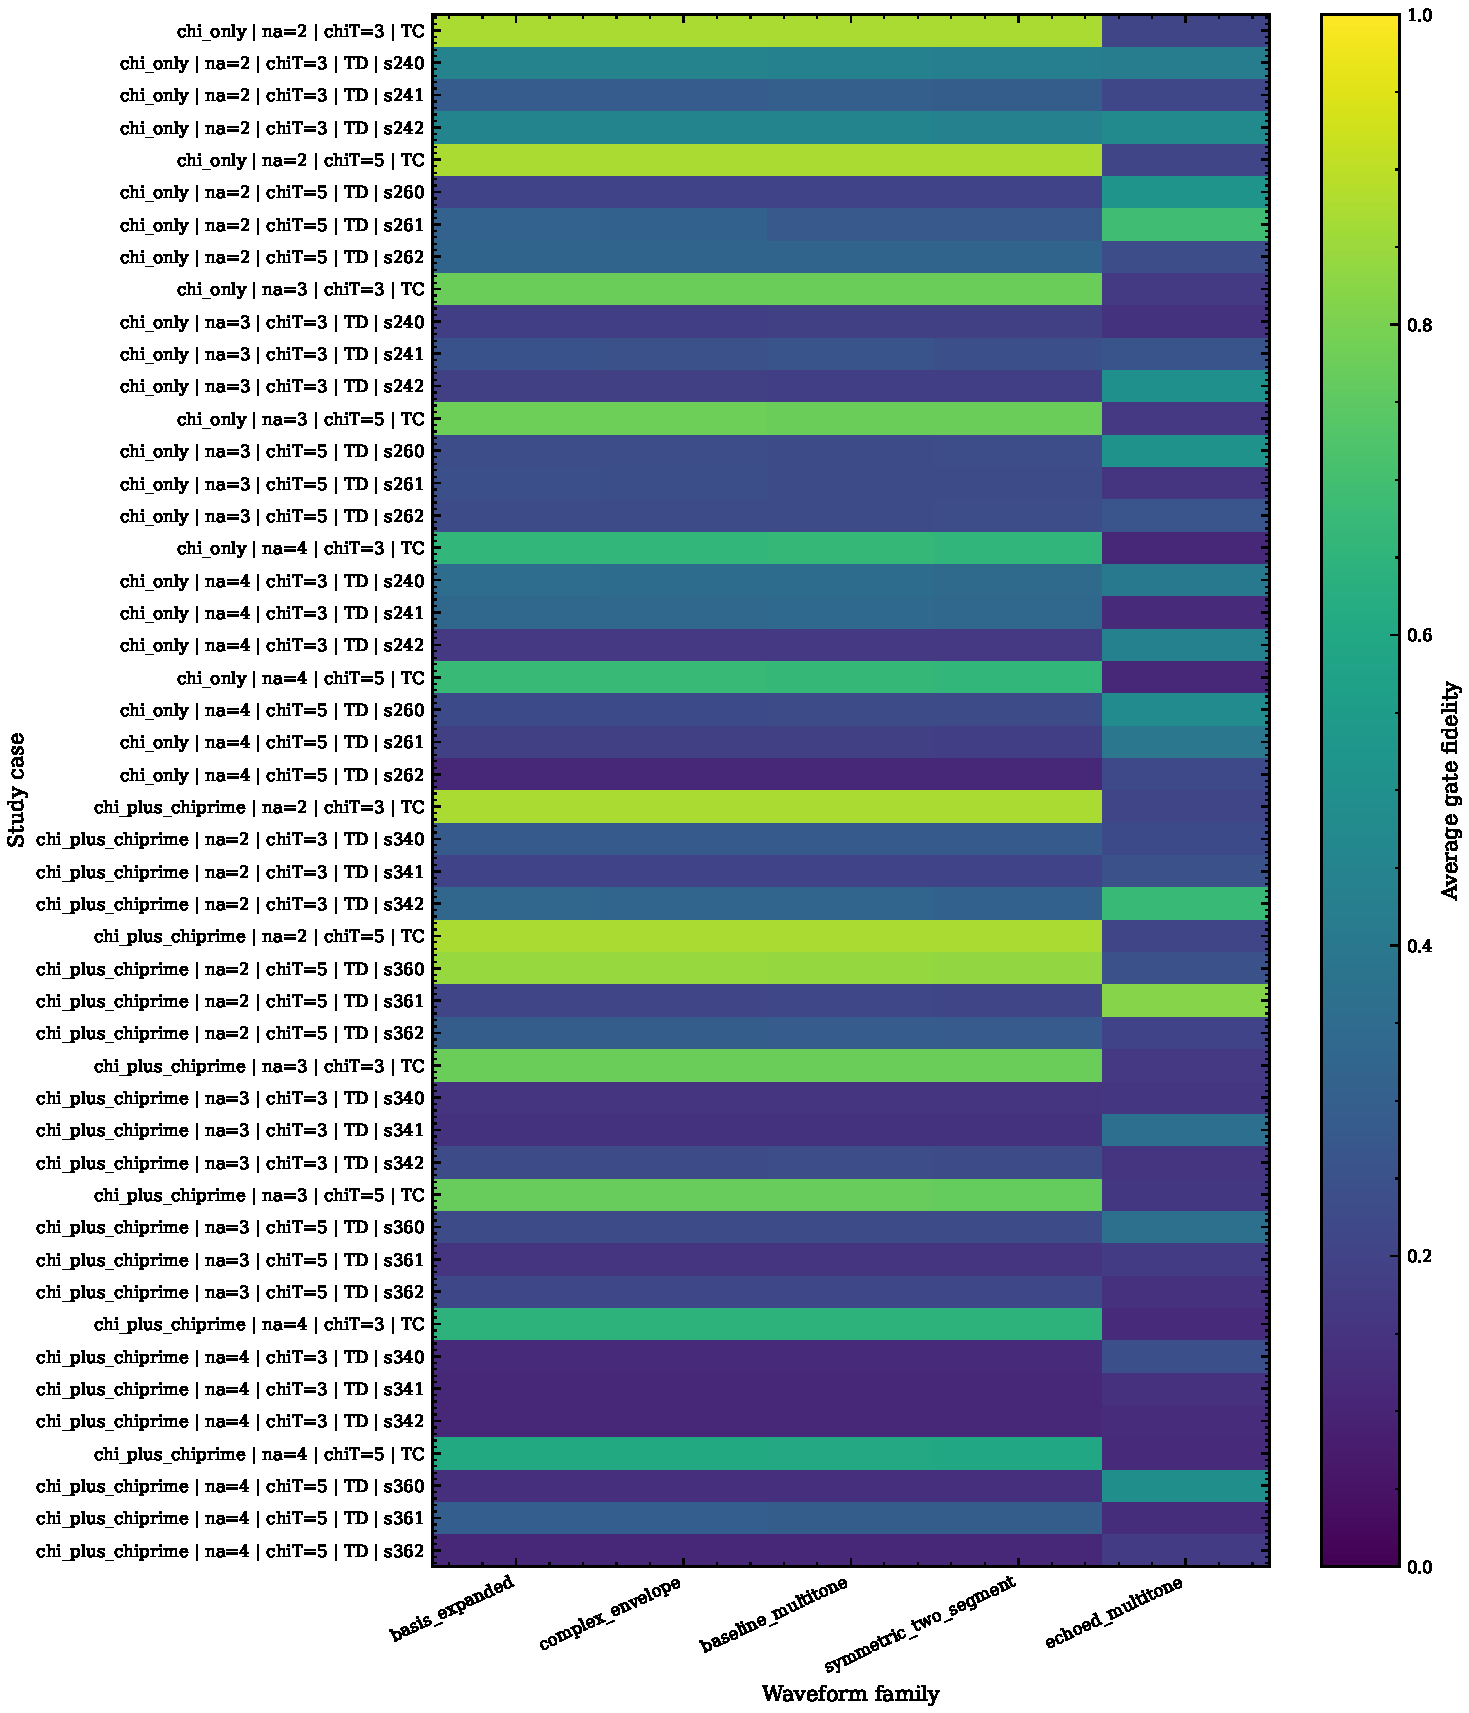
\includegraphics[width=0.9\textwidth]{../figures/case_family_fidelity_heatmap.pdf}
    \caption{Full case-by-family fidelity heatmap for the expanded sweep. The structured target rows (TC) remain high-fidelity for the baseline and the best single-segment refinements, whereas many random target rows (TD) are won by the echoed family.}
    \label{fig:appendix_heatmap}
\end{figure*}

\begin{figure}[t]
    \centering
    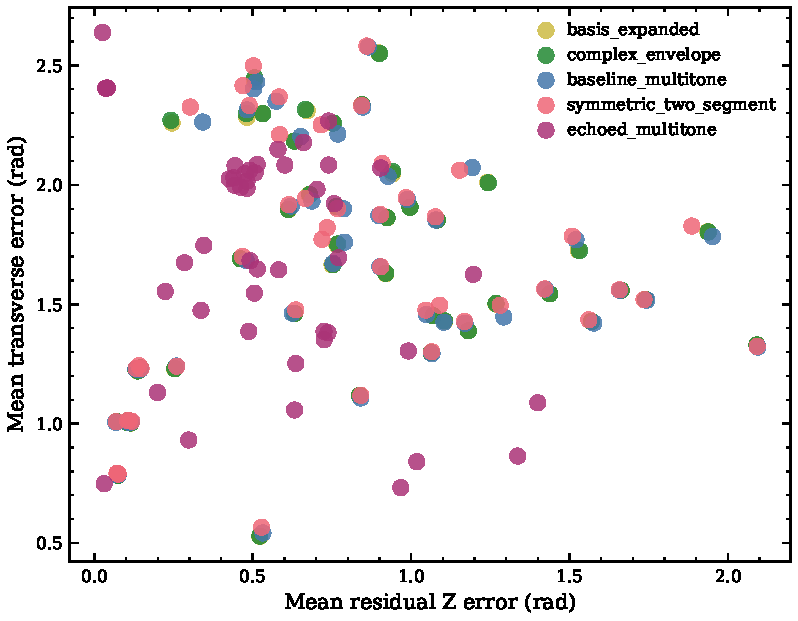
\includegraphics[width=\columnwidth]{../figures/residual_z_vs_transverse.pdf}
    \caption{Full coherent-error cloud for the expanded sweep. The echoed family occupies a distinct region with lower residual-$Z$ but widely varying transverse error, reflecting its target-class asymmetry.}
    \label{fig:appendix_errorplane}
\end{figure}

\section{Reproducibility}
\subsection{Optimized Parameters}
The richer-family optimization vectors are stored per case in \path{artifacts/cases/*.json} under the \texttt{optimizer} field. Baseline optimized tone corrections and tone specifications are stored in the same case artifacts for the baseline family.

\subsection{Waveform and Pulse Information}
Each case artifact contains sampled channel waveforms under \texttt{waveform\_samples}. Companion NPZ files are stored in \path{artifacts/waveforms/*.npz}. The echoed family contains two multitone segments plus one explicit Gaussian qubit echo pulse; the other richer families use one or two sampled multitone segments as described in the artifact metadata.

\subsection{Gate Sequence and Decomposition}
The baseline, complex-envelope, and basis-expanded families use a single conditioned multitone pulse. The symmetric family uses two equal-duration mirrored multitone segments. The echoed family uses two multitone segments separated by a Gaussian qubit $X_\pi$ pulse.

\subsection{Modeling and Simulation Assumptions}
All runs use the qubit-first convention, a two-level qubit model, fixed timestep $\Delta t = \SI{4}{ns}$, cavity truncation $N_{\mathrm{cav}} = N_{\mathrm{active}} + 2$, and a closed-system Hamiltonian with $\chi$ and optional $\chi'$ only. No decoherence or cavity self-Kerr is included in the main comparison.

\subsection{Reproduction Procedure}
Run \path{scripts/run_study.py} from the study \path{scripts/} directory to regenerate the expanded sweep. Use \texttt{--case <case\_id>} to rerun one case only. The notebook \path{scripts/reproducibility_notebook.ipynb} loads the saved study summary, figures, and case tables without rerunning the optimizer.

\subsection{Saved Artifacts}
The key saved outputs are:
\begin{itemize}
    \item \path{data/study_results.csv}: flat table of all $240$ waveform-family rows.
    \item \path{data/study_summary.json}: family-level and case-level aggregate summary.
    \item \path{data/study_summary.md}: concise human-readable summary.
    \item \path{artifacts/cases/*.json}: one JSON file per case and waveform family, including metrics, waveform samples, and optimizer metadata.
    \item \path{artifacts/waveforms/*.npz}: compact waveform sample exports for the saved cases.
\end{itemize}

\end{document}